\begin{pastexam}[label={px:df3-102-ds-06}]{地方三等資訊處理 102 年 第六題}
（申論；15 分）

在一個二元樹裡有許多節點（nodes）。假設每一個節點的資料結構如下圖：
\begin{center}
\begin{tabular}{|p{5em}|p{5em}|p{5em}|}
\hline
LEFT & DATA & RIGHT \\ \hline
\end{tabular}
\end{center}
其中 DATA 欄位為該節點的資料。LEFT 欄位為指向左方子樹的指標變數。RIGHT 欄位為指向右方子樹的指標變數。\\
如果節點 p 沒有左方子樹，其 LEFT 欄位為空指標（null pointer）。同理，如果節點 p 沒有右方子樹，其 RIGHT 欄位為空
指標（null pointer）。
\begin{itemize}[leftmargin=2.2em]
\item[㈠] 如果一個二元樹有 n 個節點，那麼它有幾個空指標？（5 分）
\item[㈡] 我們可以利用原本是空指標的欄位來儲存引線（threads）。二元樹加上引線的結果稱為引線樹（threaded trees）。
當然我們必須在各節點再加上兩個欄位 LTAG 及 RTAG，共 5 個欄位，如下圖所示：
\begin{center}
\begin{tabular}{|p{4em}|p{4em}|p{4em}|p{4em}|p{4em}|}
\hline
LTAG & LEFT & DATA & RIGHT & RTAG \\ \hline
\end{tabular}
\end{center}
如果 LEFT 欄位代表一般的節點指標，則 LTAG = 0。如果 LEFT 欄位代表引線指標，則 LTAG = 1。同理，如果 RIGHT 欄位
代表一般的節點指標，則 RTAG = 0。如果 RIGHT 欄位代表引線指標，則 RTAG = 1。\\
請將下圖的二元樹加上適當的引線指標，讓它變成引線樹，並請繪圖標出 A 到 I 共 9 個節點中所有引線指標指向的節點。
（10 分）
\begin{center}
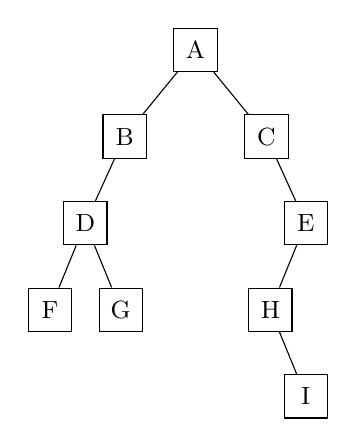
\begin{tikzpicture}[v/.style={rectangle,draw,minimum size=5.5mm,inner sep=1pt,font=\small},
  level distance=11mm, level 1/.style={sibling distance=18mm}, level 2/.style={sibling distance=10mm},
  level 3/.style={sibling distance=9mm}]
\node[v] {A}
  child {node[v] {B}
    child {node[v] {D} child {node[v] {F}} child {node[v] {G}}}
    child[missing] {}}
  child {node[v] {C}
    child[missing] {}
    child {node[v] {E}
      child {node[v] {H} child[missing] {} child {node[v] {I}}}
      child[missing] {}}};
\end{tikzpicture}
\end{center}
\end{itemize}
\end{pastexam}

\begin{pastsoln}
答案：㈠ $n + 1$ 個。 ㈡ 採中序引線：中序是 F, D, G, B, A, C, H, I, E；引線為 F.LEFT $\to$ 無（前導，指向串列頭）、
F.RIGHT $\to$ D、G.LEFT $\to$ D、G.RIGHT $\to$ B、B.RIGHT $\to$ A、C.LEFT $\to$ A、H.LEFT $\to$ C、I.LEFT $\to$ H、
I.RIGHT $\to$ E、E.RIGHT $\to$ 無（後繼，指向串列頭）。

\textbf{㈠} $n$ 個節點共有 $2n$ 個指標欄位。 除了根，每個節點恰好被它父節點的一個欄位指著，所以非空的指標有
$n - 1$ 個，空指標有 $2n - (n - 1) = n + 1$ 個（資結書第~7.5~節）。 （$n = 0$ 時沒有節點，這個式子從 $n \ge 1$ 起
適用。）本題的樹 $n = 9$，空指標應有 $10$ 個，下面的引線正好用掉這 $10$ 個欄位。

\textbf{㈡} 題目沒有指定哪一種順序的引線，這裡用最常見的\textbf{中序引線}（資結書第~7.5~節）：空的 LEFT 改指向
這個節點在中序中的前一個（前導），空的 RIGHT 改指向中序中的下一個（後繼），並把對應的 TAG 設成 $1$。

先求中序（左、根、右）：B 子樹是 F, D, G, B；C 子樹是 C，接著 E 子樹 H, I, E。 整棵樹
\[
\text{F, D, G, B, A, C, H, I, E}.
\]
逐一檢查每個空指標：
\begin{center}
\small
\begin{tabular}{lcccc}
\toprule
節點 & 空的欄位 & 中序前導 & 中序後繼 & 引線 \\
\midrule
F & LEFT, RIGHT & （無） & D & LEFT $\to$ 頭節點，RIGHT $\to$ D \\
G & LEFT, RIGHT & D & B & LEFT $\to$ D，RIGHT $\to$ B \\
B & RIGHT & & A & RIGHT $\to$ A \\
C & LEFT & A & & LEFT $\to$ A \\
H & LEFT & C & & LEFT $\to$ C \\
I & LEFT, RIGHT & H & E & LEFT $\to$ H，RIGHT $\to$ E \\
E & RIGHT & & （無） & RIGHT $\to$ 頭節點 \\
\bottomrule
\end{tabular}
\end{center}
A、D 兩個子節點都有，沒有引線。 F 是中序第一個、E 是最後一個，它們沒有前導、後繼。 這裡照很多教科書的做法（資結書第~7.5~節也介紹）加一個
\textbf{頭節點}：頭節點的 LEFT 指向根 A，F.LEFT 和 E.RIGHT 這兩條引線都指向頭節點，這樣從任何一點出發都不會碰到
空指標；若不用頭節點，這兩條引線就指向 \NIL（TAG 仍設 $1$）。 引線共 $10$ 條，正好等於 ㈠ 的 $n + 1$。

下圖實線是原本的樹枝，虛線箭頭是引線：
\begin{center}
\begin{tikzpicture}[v/.style={rectangle,draw,minimum size=6mm,inner sep=1pt,font=\small},
  t/.style={-{Latex[length=1.8mm]},dashed,thin}]
\node[v] (A) at (0,0) {A};
\node[v] (B) at (-2,-1.2) {B};
\node[v] (C) at (2,-1.2) {C};
\node[v] (D) at (-3,-2.4) {D};
\node[v] (E) at (3,-2.4) {E};
\node[v] (F) at (-3.8,-3.6) {F};
\node[v] (G) at (-2.2,-3.6) {G};
\node[v] (H) at (2.2,-3.6) {H};
\node[v] (I) at (3,-4.8) {I};
\node[v,dotted] (HD) at (0,1.3) {頭};
\draw[-{Latex[length=1.8mm]}] (HD) -- (A);
\draw (A)--(B) (A)--(C) (B)--(D) (D)--(F) (D)--(G) (C)--(E) (E)--(H) (H)--(I);
\draw[t] (F.west) to[out=150,in=180,looseness=1.1] (HD.west);
\draw[t] (F.north) to[bend left=25] (D.west);
\draw[t] (G.north) to[bend right=25] (D.east);
\draw[t] (G.east) to[bend right=30] (B.south east);
\draw[t] (B.east) to[bend right=20] (A.south west);
\draw[t] (C.west) to[bend left=20] (A.south east);
\draw[t] (H.north west) to[bend left=25] (C.south);
\draw[t] (I.west) to[bend left=25] (H.south);
\draw[t] (I.east) to[bend right=35] (E.east);
\draw[t] (E.north east) to[out=60,in=0,looseness=1.1] (HD.east);
\end{tikzpicture}
\end{center}
各節點的 TAG：A、D 的 LTAG $=$ RTAG $= 0$；B：LTAG $= 0$、RTAG $= 1$；C：LTAG $= 1$、RTAG $= 0$；E：LTAG $= 0$、
RTAG $= 1$；H：LTAG $= 1$、RTAG $= 0$；F、G、I：LTAG $=$ RTAG $= 1$。 有了引線，中序走訪不需要堆疊：從頭節點
往左一路走到 F，之後每次「RTAG $= 1$ 就直接沿引線到後繼，否則到右子樹再一路往左」即可（資結書虛擬碼~7.6）。
\end{pastsoln}
